
% HEADER
% ------------------------------------------------------------------------
% Latex - Einstellungen ***************************************************
% ------------------------------------------------------------------------
% von: Stefan Sobernig
%%%%%%%%%%%%%%%%%%%%%%%%%%%%%%%%%%%%%%%%%%%%%%%%%%%%%%%%%%%%%%%%%%%%%%%%%%
%
% ========================================================================

%% Dokumenten Klasse ===========================================================================
%
% --[ KOMA ] -----------------------------------------------------------------------------------
% Klassen: scrartcl, scrreprt, scrbook, scrletter
%  
\documentclass[%
 10pt,%           Schriftgröße
 a4paper,%	      Papier
 %DIV12,%           Seitengröße (siehe Koma Skript Dokumentation !)
 %BCOR5mm,%        Zusätzlicher Rand auf der Innenseite 
 english,%		      Sprache
 %twoside,%	      Seitenränder werden an doppelseitig angepasst
 %fleqn,%          Formeln werden linksbündig (und nicht zentriert) angezeigt 
 %openleft,%       (openright) Ein neues Kapitel beginnt immer auf einer rechten/linken Seite
 %titlepage,%      Titel wird in einer 'titlepage' Umgebung gesetzt
 %bigheadings,%    Große Überschriften (normal, small- headings)
 %halfparskip-%   Absatz wird nicht eingerückt, dafür aber um eine halbe Zeile nach unten gerückt
 %liststotoc,%     Tabellen & Abbildungsverzeichnis ins Inhaltsverzeichnis
 %bibtotoc,%       LitVerzeichnis ins Inhaltsverzeichnis
 %tablecaptionsbelow, %	Caption wird bei table unter die Tabelle gesetzt
 %headinclude,
 %nochapterprefix% Kein 'Kapitel' vor einem neuen Kapitel
 ]{scrartcl}%     Klassen: scrartcl, scrreprt, scrbook, scrletter 
% ----------------------------------------------------------------------------------------------

%% Alles was vor alles andere gehört.... =======================================================
%
%
\usepackage{calc} % Zum Rechnen innerhalb von Latex
%
% ----------------------------------------------------------------------------------------------

%% Schriften ===================================================================================
%
% -- Andere Schriftpakete -----
%
% - Times, Helvetica, Courier (Word Standard...)
%\usepackage{mathptmx}
%\usepackage[scaled=.90]{helvet}
%\usepackage{courier} 
% statt courier man kann auch die Standardschrift cmtt beibehalten
% -------------------
%
% - Palantino , Helvetica, Courier 
%\usepackage{mathpazo}
\usepackage[scaled=.92]{helvet}
%\usepackage{courier} 
% -------------------

% Weitere Times Schriften
%\usepackage{utopia}
%\usepackage{charter}
% Serifenlose Schrift
%\usepackage{avant}
% -----------------------------
%
% -- Koma Schriften --
%\renewcommand*{\headfont}{\small\sffamily\slshape}        % Kopfzeile
%\renewcommand*{\pnumfont}{\bfseries\sffamily}             % Seitenzahl
%\setkomafont{chapter}{\sffamily\Huge}                     % Chapter
%\renewcommand*{\sectfont}{\sffamily} %\rmfamily\bfseries  % Titelzeilen
%\renewcommand*{\capfont}{\small}                          % Schrift für Caption
%\renewcommand*{\caplabelfont}{\sffamily\bfseries\small}   % Schrift für 'Abbildung' usw.
%
% -- Schriften für Caption's von _nicht_- Koma kompatiblen Paketen
%
% Bei verwendung von Caption2 treten Komplikationen mit Koma auf. 
% Diese Korrekturren sind hier noch nicht implementiert !
%
%\usepackage{caption2}
%\renewcommand{\captionfont}{\small}
%\renewcommand{\captionlabelfont}{\sffamily\bfseries\small}
%\captionstyle{flushleft}
%
% -- Setzen der Titelzeile --
%\renewcommand*{\raggedsection}{\raggedright} % linksbündig, hängend
%\renewcommand*{\raggedsection}{} % Blocksatz (Latex-Standart)
%
% ----------------------------------------------------------------------------------------------
% *** Sprache *****************************
\usepackage[english]{babel}
\usepackage[T1]{fontenc}
\usepackage[latin1]{inputenc}
%------------------------------------------
% Bibliographie-Stil ===========================================================================
%\usepackage{natbib}
%\bibliographystyle{dinat}
%% Seitenlayout ================================================================================
%
% Layout laden um im Dokument den Befehl \layout nutzen zu können
%\usepackage[verbose]{layout} 
%
% Optischer Randausgleich (geht nur mit pdflatex, ansonsten hat es keine Auswirkung)
%\usepackage[activate=normal]{pdfcprot} 

% 1. Layout mit 'typearea'
% hier werden die Optionen aus \documentclass[] angewandt !
%\usepackage{typearea}

% 2. Alternative: Layout mit 'geometry'
%\usepackage{geometry}
%\geometry{a4paper}
%\geometry{twoside}
%\geometry{marginparwidth=85pt}
%\geometry{textheight=55\baselineskip}
%\geometry{textwidth=418pt} % Standard
%\geometry{bindingoffset=5mm}
%
% - Anzeigen des Layouts -
%\geometry{showframe}

% -- Zeilenabstand --
%\usepackage{setspace}
%\doublespace	        % 2-facher Abstand
%\onehalfspace        % 1,5-facher Abstand

% -- Kopfzeilen ---
\usepackage[automark, nouppercase]{scrpage2}
% Seite mit Headern
\pagestyle{scrheadings}
%
% löscht voreingestellte Stile
%\clearscrheadings 
%\clearscrplain
%
% Was steht wo...
%\ohead{\pagemark} % Oben außen: Seitenzahlen
%\ihead{\headmark} % Oben innen: Setzt Kapitel und Section automatisch
%\rehead{\leftmark} %Oben links: Kapitel
%\lohead{\rightmark} %Oben rechts: Section
%\cfoot[\pagemark]{} % Mitte unten: Seitenzahlen bei plain
\ofoot[]{\pagemark} % Mitte unten: Seitenzahlen bei headings
% Angezeigte Abschnitte im Header
%\automark[section]{chapter} %[rechts]{links}
%\automark[subsection]{section} %[rechts]{links}
% 
% Linien
%\setheadsepline{.4pt} % Linie unter dem Head
%setheadtopline{2pt} % Ganzoben
%\setfootbotline{.4pt} % Ganzunten
%
% Wie weit geht die Kopfzeile...
%\setheadwidth[0pt]{textwithmarginpar}
%\setheadwidth[0pt]{text} % standard
%
% Schriftformatierung der Kopfzeile
%\setkomafont{pagehead}{\normalfont\normalcolour\small}
%\setkomafont{pagenumber}{\normalfont\normalcolour\small}
% -- Fußnoten ---
%\deffootnote{1.5em}{1em}{
%\textsuperscript{\thefootnotemark}
%------------------------------------------
%
% ----------------------------------------------------------------------------------------------

%% sonstige Einstellungen ======================================================================
%
%-- Alternativer Absatz --
%\setlength{\parindent}{0pt} % Einzug = 0
% Siehe auch KOMA Skript zu den dortigen M�glichkeiten !!

% -- Setzen von Abbildungsbeschreibungen --
%\setcapindent*{1em} % siehe Komadokumentation Abschnitt 3.5
\setcapindent{1em} 
\addtokomafont{caption}{\scriptsize}
%
% *** Inhaltsverzeichnis ******************
\setcounter{secnumdepth}{3}  % Abbildungsnummerierung mit größerer Tiefe
\setcounter{tocdepth}{3}		 % Inhaltsverzeichnis mit größerer Tiefe
%------------------------------------------
%
% -- Ändern von Titeln --
%\usepackage{titlesec}
%\titlelabel{\thetitle.\quad} % Einen Punkt an alle Nummerierungen anfügen
%
% ----------------------------------------------------------------------------------------------

%% Bilder und Graphiken ======================================================================

% *** Bilder ******************************
% Grundlegendes
\usepackage[final]{graphicx}  % enth�lt \includegraphics !!
%\usepackage[draft]{graphicx} % Option: 'draft' für das _nicht_ Einbinden von Bildern
%\usepackage{subfigure}        % Bilder nebeneinander 
%
% Erweiterungen
%\usepackage{picinpar}         % Befehl: 'window' zum Setzen von Bildern neben Text
%
\usepackage{float}            % Stellt die Option [H] für Floats zur Verf�gung 
%\usepackage[rflt]{floatflt}   % Stellt Befehlt 'floatingfigure' zur Verf�gung
                              % [rflt] - Standard float auf der rechten Seite
%-------------------------------------------
%
% - Color Paket für farbigen Text --> _VOR_ pstricks/pst-plot !! ---
\usepackage{color} 
% Beispiel für neue Farbe: \definecolor{meingrau}{gray}{0.90}
% ------------------------------------------------------------------

% *** Graphen ******************************
\usepackage{pst-plot}
%\usepackage{psfrag}
%-------------------------------------------
%
% ----------------------------------------------------------------------------------------------


%% Mathe =======================================================================================

% *** Mathematik **************************************
%
% Neue Mathebefehle 
%\usepackage{amsmath} % der QUASI-STANDARD 
% den Befehl: eqnarray hiernach _nicht_ mehr verwenden
%------------------------------------------------------

% -- Symbole ---------
%\usepackage{amssymb}
\usepackage{latexsym} 
%\usepackage{wasysym} % (für \varangle)
%---------------------
%
% ----------------------------------------------------------------------------------------------

%% sonstige Pakete =============================================================================
%
\usepackage{makeidx}		% Index
%\usepackage{minitoc}    % Mini TOC's vor jedem Kapitel
%
\usepackage{enumerate}  % Optionen [a)], [i)] usw. 
%
%\usepackage{array}
\usepackage{tabularx}   % Erweiterte Tabellen Optionen
\usepackage{multirow} 
%
%\usepackage{fancybox}   % für shadowbox, ovalbox
\usepackage{ulem}       % Zum Unterstreichen (z.B. Tensor)
\usepackage{textcomp}
\renewcommand{\familydefault}{\sfdefault}  % Symbole - z.B. \copyright
\usepackage{xspace}
% ----------------------------------------------------------------------------------------------

%% Eigene Definitionen =========================================================================
%

% tex4ht settings
%\usepackage[xhtml]{tex4ht} 

\usepackage{listings} % allows for including code listings similar to \verbatim and \verb
\lstset{rangeprefix=\#<\ ,% curly left brace plus space 
rangesuffix=\ >\#,%
includerangemarker=false}% space plus curly right brace

%
% ----------------------------------------------------------------------------------------------

% -- Auszuführende Befehle (vor Dokument Beginn) ----
%\makeindex
%\dominitoc
% ---------------------------------------------------

\usepackage[numbers]{natbib}
\bibliographystyle{plainnat}

% support for embedded xmp
\ifpdfoutput{
  \usepackage{hyperref}% generates in-document hyper references from \ref and \label
  \definecolor{darkblue}{rgb}{0,0,.5}
  \hypersetup{colorlinks=true, breaklinks=true, linkcolor=darkblue,
    menucolor=darkblue, pagecolor=darkblue, urlcolor=darkblue,
    citecolor=darkblue}
  \usepackage{xmpincl}
  \usepackage[nofancy]{svninfo}
  \cfoot[]{\svnInfoFile, rev. \svnInfoRevision, \svnInfoDate}
  \newcommand{\site}{http://alice.wu-wien.ac.at:8000}
  }{
  \newcommand{\site}{}
  % \DeclareGraphicsRule{.png}{png}{.bb}{}%
}

% display svn info


% booktabs, longtable
\usepackage{booktabs}
\usepackage{longtable}

\newenvironment{hints}{\begin{itemize}\renewcommand\labelitemi{$\hookrightarrow$}\footnotesize}{\end{itemize}}
%\newcommand{\apilink}[3]{\href{{http://localhost:8000/api-doc/proc-view?proc=}#1+#2+#3}{#1\rightarrow#3}}
\newcommand{\acsapi}{\site/api-doc}
\newcommand{\xotclapi}{\site/xotcl}
\newcommand{\xotcl}{http://media.wu-wien.ac.at/langRef-xotcl.html}
\newcommand{\proclink}[3]{\href{\acsapi/proc-view?proc=#1+#2+#3}{#1\begin{math}\rightarrow\end{math}#3}}
\newcommand{\objlink}[1]{\href{\xotclapi/show-object?object=#1}{#1}}
\newcommand{\xotclref}[2]{\href{\xotcl\##1}{#2}}
\newcommand{\filelink}[2]{\href{\acsapi/procs-file-view?path=packages/#1}{#2}}
\newcommand{\xsd}[1]{\href{http://www.w3.org/TR/xmlschema-2/\##1}{xsd:#1}}











% MAIN 
%body
% embed by-sa metadata file
\includexmp{by-sa-2.0}
\makeindex
  \begin{document}
  \svnInfo $Id$
%titlepage
\title{Request brokerage and remoting for OpenACS}
\author{Stefan Sobernig}
\date{July 2007}
\maketitle
%body

     \section{Introduction}
        \textbf{xorb}, the X(OTcl) R(equest) B(roker) (OpenACS package key: xotcl-request-broker), is an 
infrastructure package for the web development toolkit OpenACS and OpenACS-based frameworks that 
provides for generic means of call abstraction.  Call abstraction, hereby, refers to both distributed and 
non-distributed scenarios. In a non-distributed scenario, xorb is an object-oriented refinement of the well 
established OpenACS facilities also referred to as 'service contracts'. In a distributed scenario, xorb 
provides a remoting infrastructure for OpenACS. xorb was designed in a protocol-agnostic manner, i.e. 
our primary intention is to provide support for a variety of remoting protocols. Protocol support is, 
therefore, realised in terms of protocol plug-ins for xorb. So far, we have realised a feature-rich SOAP 
protocol plug-in referred to as \textbf{xosoap} (OpenACS package key: xotcl-soap).

This guide, in its current shape, aims at providing the fundamentals of using call abstractions in a 
distributed scenario. We restrict ourselves, for the moment, to the remoting capabilities and therefore 
introduce the reader to the SOAP protocol plug-in, i.e. xotcl-soap (xosoap). The present document and 
resource collection will be steadily extended to cover more general aspects of request brokerage and 
protocol plug-ins available.
\subsection{Sources of information}
Beyond this manual, the following materials are currently available.
\begin{itemize}
\item A \href{http://openacs-dotlrn.wu-wien.ac.at}{wiki version of this manual}, allowing for commenting 
publicly and writing ahead.
\item We aim at documenting elements of the public interfaces by means of the OpenACS in-code 
documentation facility and the API Browser. References will be given throughout the manual where 
appropriate.
\item Tutorial prepared for the \href{http://oacs-dotlrn-conf2007.wu-wien.ac.at/}{OpenACS Spring 
Conference 2007} (up-to-date):
\begin{itemize} 
\item \href{http://oacs-dotlrn-conf2007.wu-wien.ac.at/conf2007/file/sobernig-xosoap-slides.pdf?
m=download|Slide set}{Slide set}
\item A \href{http://oacs-dotlrn-conf2007.wu-wien.ac.at/conf2007/file/tutorial-sobernig.mp4?
m=download}{podcast recording} of my talk
\end{itemize}
\item \href{http://nm.wu-wien.ac.at/research/publications/b670.pdf}{Tutorial (slide set)} prepared for the 
OpenACS Fall Conference 2006 (obsolete) 
\end{itemize}
Please, note that these resources reflect and document various stages of development and don't 
necessarily reflect the current state. The only source of information that is kept up-to-date is this manual 
document and its wiki mirror. Moreover, some of them might focus advanced concepts that are properly 
elaborated in the realm of this general-purpose documentation.
\subsection{Copyright terms}
The XOTcl Request Broker (xorb) and all protocol plug-in packages, i.e. currently xosoap, are provided 
under the provisions of the \href{http://creativecommons.org/licenses/LGPL/2.1/}{Lesser General Public 
License (LGPL) version 2.1}. All accompanying and documentary work, including this document, comes 
under the \href{http://creativecommons.org/licenses/by-sa/2.0/at/}{Creative Commons Attributation and 
Share-alike (by-sa) licence}.

     \section{Installation \& configuration guideline}
     	\subsection{Prerequisites}
	\subsection{The XOTcl Request Broker (xorb)}
 
	\subsection{The SOAP protocol plug-in (xosoap)}
  \section{A quick start guide}\label{sec:quickstart}
  \subsection{xorb}\label{sec:quickstart:xorb}
  \subsection{xosoap}\label{sec:quickstart:xosoap}
  The aim of this quick start section is to provide you with all the critical information required to get you 
started with integrating SOAP in your OpenACS application in terms of consuming an existing SOAP 
service and providing your own as quick as possible. We provide ready-made and take-away code 
snippets and discuss the important steps in further detail. At some point, we might refer to further 
readings or more advanced concepts. 
  \subsubsection{How to glue to ...?}\label{sec:xosoap:quickstart:glueto}
  Say, you want to realise a scenario as depicted in Figure \ref{fig:quickstart:xosoap:1}, i.e. you want to 
use the simple echo functionality provided by a remote object or remote procedure through SOAP. In this 
example scenario, we take a remote SOAP service called EchoService as a given. It might realised 
either in xosoap itself or any other SOAP infrastructure framework, such as gSOAP, Apache Axis, .NET 
Remoting and the like. Further, we assume that  EchoService features a call 'echoFloat' that requires a 
single argument of type 'float' (as defined as 'built-in' simple type by the XML schema specification) as 
input and promises to return a value of the very same type. How do you call and consume this little 
example SOAP service by means of xosoap?
\begin{figure}[htbp]
\begin{center}
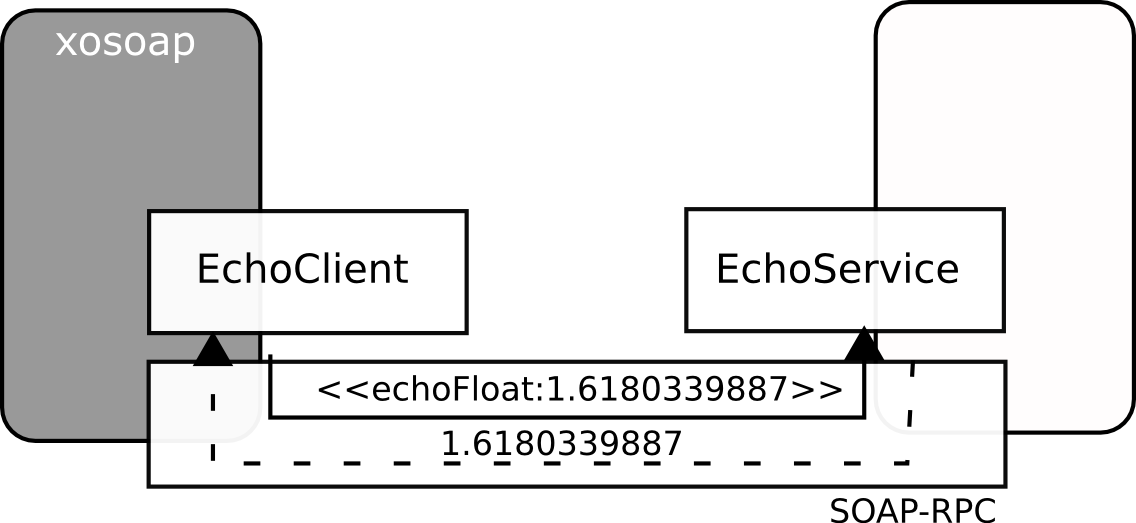
\includegraphics[width=0.5\textwidth]{img/consumer.png}
\caption{Our example scenario}
\label{fig:quickstart:xosoap:1}
\end{center}
\end{figure}
\begin{hints}
\item Hold on! If you prefer to skip the little code walk below, just look at the underlying and deployable 
example script xotcl-request-broker/www/doc/manual/examples/xosoap/example-01-soap-consumer.tcl 
or \href{http://openacs-dotlrn.wu-wien.ac.at/request-broker/doc/manual/examples/xosoap/example-01-
soap-consumer.tcl}{direct your browser to it} to see it at work.
\item xosoap's public interface comes with a few flavours to realise soap clients: \nameref
{sec:advanced:interface:what}
\end{hints}
You just need four little steps and a few lines of code to get there:
\begin{enumerate}
\item Provide SOAP-specific configuration information as \emph{glue object}. To be concrete, create an 
instance of the XOTcl class ::xosoap::SoapGlueObject and initiate the newly created object with some 
important bits of information:
\lstinputlisting[breaklines=true,numbers=left,frame=single,basicstyle=
\footnotesize,firstline=6,lastline=10]{../examples/xosoap/example-01-soap-consumer.tcl}
In these four lines, we create and initiate an instance of the glue object class and provide three 
information items to it. In line 2, we pass the actual endpoint address. In a conventional setting, the 
transport endpoint corresponds to a valid unique resource identifier (URL) as required by the HTTP 
protocol as transport provider. Line 4 also meets an information requirement at the HTTP level, i.e. the 
value assigned to a specific HTTP header field prescribed by SOAP 1.1/1.2 specifications: the 
SOAPAction header field. Line 2 and the setter call on callNamespace, on the contrary, refers to a higher 
protocol level, i.e. the SOAP level. The value of callNamespace will be used to set the namespace 
attached to the method-describing element. This is used by a few SOAP frameworks, e.g. .NET 
Remoting, to dispatch the remote call correctly to the responsible servant. For a detailed list of 
configuration options, please, refer to ::xosoap::SoapGlueObject.

Want to learn more?
 \begin{hints}
\item \nameref{sec:advanced:xorb:gobjects:what}
% context object > principles of argument parsing
\item \nameref{sec:advanced:xorb:gobjects:why}
% concatenation of shadow information
\end{hints}

\item Create a local proxy of the remote object or remote procedure, a so called \emph{client proxy}
\index{Clientproxy}. This client proxy object holds a proxy method for the remote method or procedure to 
call. There are a few flavours for specifying such a client proxy, the most straight forward, however, is by 
instantiating ::xorb::ProxyObject and thus creating a proxy object (ProxyObject might be resolved as 'G
(lueing)Object' which introduces a subtle difference between glue object and glueing object).
\lstinputlisting[breaklines=true,numbers=left,frame=single,basicstyle=
\footnotesize,firstline=13,lastline=13]{../examples/xosoap/example-01-soap-consumer.tcl}
The only significant action here is to associate the previously defined glue object to the client proxy. The 
information encapsulated by the glue object is then used by the underlying infrastructure to form remote 
calls out of the combined information of the glue object and the client proxies interface. The latter is 
defined in the third step.
\item Specify and realise the interface of your client proxy. The notion of object interfaces, to keep it 
simple, refers to the set methods and their method signatures defined on the object. When looking at 
Figure \ref{fig:quickstart:xosoap:1}, we learn that the interface of the remote object EchoService is quite 
simplistic: There is a single method echoFloat that takes a single argument flagged "inputFloat". The 
argument is, apart from a concrete label, further qualified by a type constraint called xsFloat. These type 
constraints are realised as \href{http://media.wu-wien.ac.at/doc/tutorial.html#non-pos-args}{check 
options on non-positional arguments}, in XOTcl terms. Besides, the interface promises a specific return 
value type, stipulated by setting "-returns" on ad\_proc.
\lstinputlisting[breaklines=true,numbers=left,frame=single,basicstyle=
\footnotesize,firstline=16,lastline=21]{../examples/xosoap/example-01-soap-consumer.tcl}
The method ad\_proc that comes with ::xorb::ProxyObject overloads ad\_proc as defined 
on ::xotcl::Object and allows for declarations of the following term structure: \\\begin{footnotesize}\textbf
{<ProxyObject>} \textbf{ad\_proc} [-returns \textit{Anything}] \textbf{<name>} \textbf{<arguments>} \textbf
{<documentation>} \textbf{<body>}\end{footnotesize}\\
For a detailed description see \apilink{::xorb::ProxyObject}{instproc}{ad\_proc}.
%\href{http://openacs-dotlrn.wu-wien.ac.at/api-doc/proc-view?proc=::xorb::ProxyObject+instproc+ad_proc}{::xorb::ProxyObject->ad\_proc}.
\item Invoke the proxy method to perform the remote call
\lstinputlisting[breaklines=true,numbers=left,label=lst:quickstart:xosoap:1,frame=single,basicstyle=\footnotesize,firstline=23,lastline=23]{../examples/xosoap/example-01-soap-consumer.tcl}
\end{enumerate}
So far, it needed three declarative steps to realise a call to a SOAP service. The public interface of 
xosoap comes with various levels of granularity (see \ref{sec:advanced:interface:what}) with the above 
example referring to the medium-level interface. The higher-level one allows to realise the previous 
example in a total of three steps with only two declarative ones. Let's rewrite the example:

\begin{enumerate}
\item The major difference is that step 1 and 2 of the previous procedure are merged into one single 
step. Note, that we now take advantage of a construct that natively comes with xosoap, the 
class ::xosoap::client::SoapObject. This makes it completely sufficient, for instance, to import from the Tcl 
namespace ::xosoap::client::* without any need to use facilities of xorb directly (see full code snippet of 
the following example in listing \ref{lst:quickstart:xosoap:3}.)
\lstinputlisting[breaklines=true,numbers=left,frame=single,basicstyle=\footnotesize,firstline=5,lastline=9]
{../examples/xosoap/example-02-soap-consumer.tcl}
\item The second step is, again, devoted to the declaration of the actual proxy interface, a local 
realisation of the echoFloat method on our combined proxy client and glue object:
\lstinputlisting[breaklines=true,numbers=left,frame=single,basicstyle=
\footnotesize,firstline=12,lastline=18]{../examples/xosoap/example-02-soap-consumer.tcl}
\item Finally, once the above is done, you can continue by issuing the call, i.e. invoke on the 'remote' 
method:
\lstinputlisting[breaklines=true,numbers=left,frame=single,basicstyle=
\footnotesize,firstline=21,lastline=21]{../examples/xosoap/example-02-soap-consumer.tcl}
\end{enumerate}

 \begin{hints}
\item See the complete example: Listing \ref{lst:quickstart:xosoap:3}.
\item See: \nameref{sec:advanced:interface:what}
\end{hints}

  
  \subsubsection{Getting glued to ...?}
  In this section, we will briefly look at some straight-forward ways to expose your OpenACS code as a 
SOAP-based service. For this very purpose, we, again, consider the scenario as introduced in the 
previous section, but this time, we shift focus. Now, we want xosoap to realise the EchoService, the 
callee, and not, as previously, the EchoClient, i.e. the caller. Figure \ref{fig:quickstart:xosoap:2} indicates 
that we now aim at realising a service that offers a single remote method, i.e. "echoFloat", that takes a 
single argument of type "float" (again, as prescribed by the XML schema specfication) and is to echo the 
value of the argument back to the caller, again as XML schema built-in "float". The service laterally 
reverses the scenario in the previous section (see \nameref{sec:xosoap:quickstart:glueto}). How can you 
achieve this?

\begin{enumerate}
\item Declare and deploy an \emph{interface description}. In OpenACS, interface descriptions have a long-standing tradition, however, sometimes neglected. You might be familiar with or, at least, you might have heart of \emph{service contracts} as provided by the OpenACS core. If not, don't panic! For the time being, you just need to know that there is something called "service contract" in OpenACS, that xorb builds upon this core feature of OpenACS and that you now need to create such a service contract, weird enough. Think of an interface description as a fundamental sketch of an object interface that lays down how the interface of a remote object and the interfaces of client proxies mimicking this remote object are to be construed. As for the EchoService in Figure \ref{fig:quickstart:xosoap:2}, a description might look the following way:
\lstinputlisting[breaklines=true,numbers=left,frame=single,basicstyle=
\footnotesize,firstline=9,lastline=23]{../examples/xosoap/example-07-soap-provider-init.tcl}
The above statement is, in the very literal sense of the word, a "blue print" for the EchoService service. Apart from a few bits of information targeting you as developer, it outlines that any servant or client proxy is meant to implement a method called "echoFloat", accepting a single argument and, in particular, throwing back a return value of a specific type. Don't forget to "deploy" your newly created service contract by calling:
\lstinputlisting[breaklines=true,numbers=left,frame=single,basicstyle=
\footnotesize,firstline=26,lastline=26]{../examples/xosoap/example-07-soap-provider-init.tcl}
This separate step of deployment might seem an overhead in this simple example, but it renders useful when considering more complex scenarios of designing and lifecycling interface descriptions.
\item Provide servant code and register it with the invocation mechanism. The lines above are, as the notion of "interface description" implies, are mere description of something. What about the realisation of that something, i.e. the actual code block that is executed when the service is called. We refer to this code artefact as servant code or \emph{servant}, in short. But simply creating servant code is not enough, you still have to let xorb know which code block to invoke when calls from client proxies occur. The latter is referred to as providing a "service implementation", i.e. registering your code piece as realisation of a specific service contract! Behind the scenes and in some use cases, it might be more appropriate to deal with these two steps separately, however, in a straight-forward "get-me-a-soap-service" scenario, xorb provides a short cut to accomplish both in a single step:
\lstinputlisting[breaklines=true,numbers=left,frame=single,basicstyle=
\footnotesize,firstline=30,lastline=38]{../examples/xosoap/example-07-soap-provider-init.tcl}
\lstinline[frame=single]!-implements! identifies the service contract realised by the underlying servant code, while \lstinline[frame=single]!-using! allows for specifying the intended delegations, which concrete code block is meant to be called for which abstract call. In our concrete example, we both provide a servant method called echoFloat and, behind the scenes, this servant method is registered as callee for abstract calls on echoFloat as defined by the contract. Note that the facility  \lstinline[frame=single]!Method! is actually an XOTcl object (i.e. a slot object, to be more precise) that mimics the declaration of instprocs and procs as known from XOTcl. Finally, also deploy your service implementation:
\lstinputlisting[breaklines=true,numbers=left,frame=single,basicstyle=
\footnotesize,firstline=41,lastline=41]{../examples/xosoap/example-07-soap-provider-init.tcl}
At this point, you have accomplished most of the work needed to provide your EchoService. Two things remain to be done:
\begin{hints}
\item Interested in some background reading on OpenACS's service contracts? See the section on \nameref{sec:internal:contracts}.
\item See the complete Listing \ref{}.
\end{hints}
\item You might have asked yourself, while going through step 1 and 2, where to actually put your the code outline above. Well, there are several answers to this question, you may choose between the following options:
\begin{itemize}
\item Your package's library files (*-procs.tcl, *-init.tcl): Preferably, drop your code in files situated in the tcl-subdirectory of your package. In either case, whether you choose a *-procs or a *-init file, make sure that you place the following line before the actual code block depicted in step 1 and 2:
\lstinline!::xo::db::package require xotcl-request-broker!. Besides, there is a subtle difference between the *-procs and *-init files. The latter are evaluated only once, during server start-up. This means, contracts and implementations are only evaluate once. If you constantly develop, let's say, the servant code declared by your implementation, and you want your modifications/ improvements to take effect without a dedicated server re-start, go for the *-procs option. This way, you can take advantage of xorb's reload and watch features.
\item Your package's W(eb) U(user) I(nterface) files: In principle, you can specify a contract (::xorb::ServiceContract) in one of your www-subdirectory files as well. While it limits their usage, it does not break any functionality. Implementations (::xorb::ServiceImplementation) might as well be specified in WUI files, however, only the most basic variant makes sense in this context. The code of step 2 would not make sense as it defines servant code as well which should be available for all connections, i.e. in the context of all connection threads, and not only the one you specified it in by calling the WUI file.
\item Developer shell: You can also drop the code in the shell as provided by the Developer Support package, however, the limitations for WUI scripts apply here as well.
\end{itemize}

\end{enumerate}
  \begin{figure}[htbp]
\begin{center}
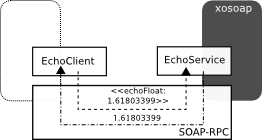
\includegraphics[width=0.5\textwidth]{img/provider.png}
\caption{Our example scenario -- The provider side}
\label{fig:quickstart:xosoap:2}
\end{center}
\end{figure}
  \section{Advanced usage}\label{sec:advanced}
    \subsection{Public interface}
  \subsubsection{What is the structure of xorb's and xosoap's public interfaces?}\label{sec:advanced:interface:what}
  As can be seen from Figure \ref{fig:advanced:interface:1}, the interface available is organised in three 
packages and at the same time levels of granularity. The \emph{lowest-level interface} is deeply 
integrated with XOTcl idioms, especially ::xotcl::Object and ::xotcl::Class. xorb, therefore, allows to turn 
any XOTcl object into a client proxy to take advantage of call abstractions (either in a distributed or non-
distributed scenario). At this level, xorb introduces two particular keywords (i.e. methods) that allow to 
define "stub" methods in the literal sense of the word on ::xotcl::Object and its subclasses, \emph{glue} 
(or \emph{ad\_glue}). These methods appear as keywords (one might refer to modifiers, though this is 
not appropriate strictly speaking) to ordinary proc or instproc declarations, however, these method 
declaration don't require or allow method bodies to be defined. The example provided in the quickstart 
guide (see \ref{sec:quickstart:xosoap} can be realised with any XOTcl object, by simply writing:
  \begin{enumerate}
\item First, again, create a 'glue' object and pass the necessary call information: \lstinputlisting[breaklines=true,numbers=left,frame=single,basicstyle=\footnotesize,firstline=6,lastline=10]{../examples/xosoap/example-03-soap-consumer.tcl}
\item In this step, you can, thanks to the deep integration with the fundamental idiom ::xotcl::Object, you 
can simply revert to the use of an ordinary object. Either create one (as shown in the example below) or 
use existing objects and make them proxy objects by, first, attaching the glue object to it and, second, 
declare a proxy interface by means of \emph{ad\_glue} (or glue):
\lstinputlisting[breaklines=true,numbers=left,frame=single,basicstyle=\footnotesize,firstline=13,lastline=13]{../examples/xosoap/example-03-soap-consumer.tcl}
\lstinputlisting[breaklines=true,numbers=left,frame=single,basicstyle=\footnotesize,firstline=17,lastline=23]{../examples/xosoap/example-03-soap-consumer.tcl}
\item The actual call is effectuated the same way as in the previous example:
\lstinputlisting[breaklines=true,numbers=left,frame=single,basicstyle=\footnotesize,firstline=26,lastline=26]{../examples/xosoap/example-03-soap-consumer.tcl}
  \end{enumerate}
At this level, stub (or proxy) methods appear in their purest forms as mere placeholders for remote calls 
realising a local representation of a remote (object) interface. Please note that declarations by means of 
glue/ ad\_glue don't take a method body as they are mere interface descriptors. This makes them 
syntactically comparable to the \xotclref{Object-abstract}{abstract keyword} that comes with XOTcl to 
mimic abstract classes. However, do not align them at the semantic level.
  \begin{figure}[htbp]
\begin{center}
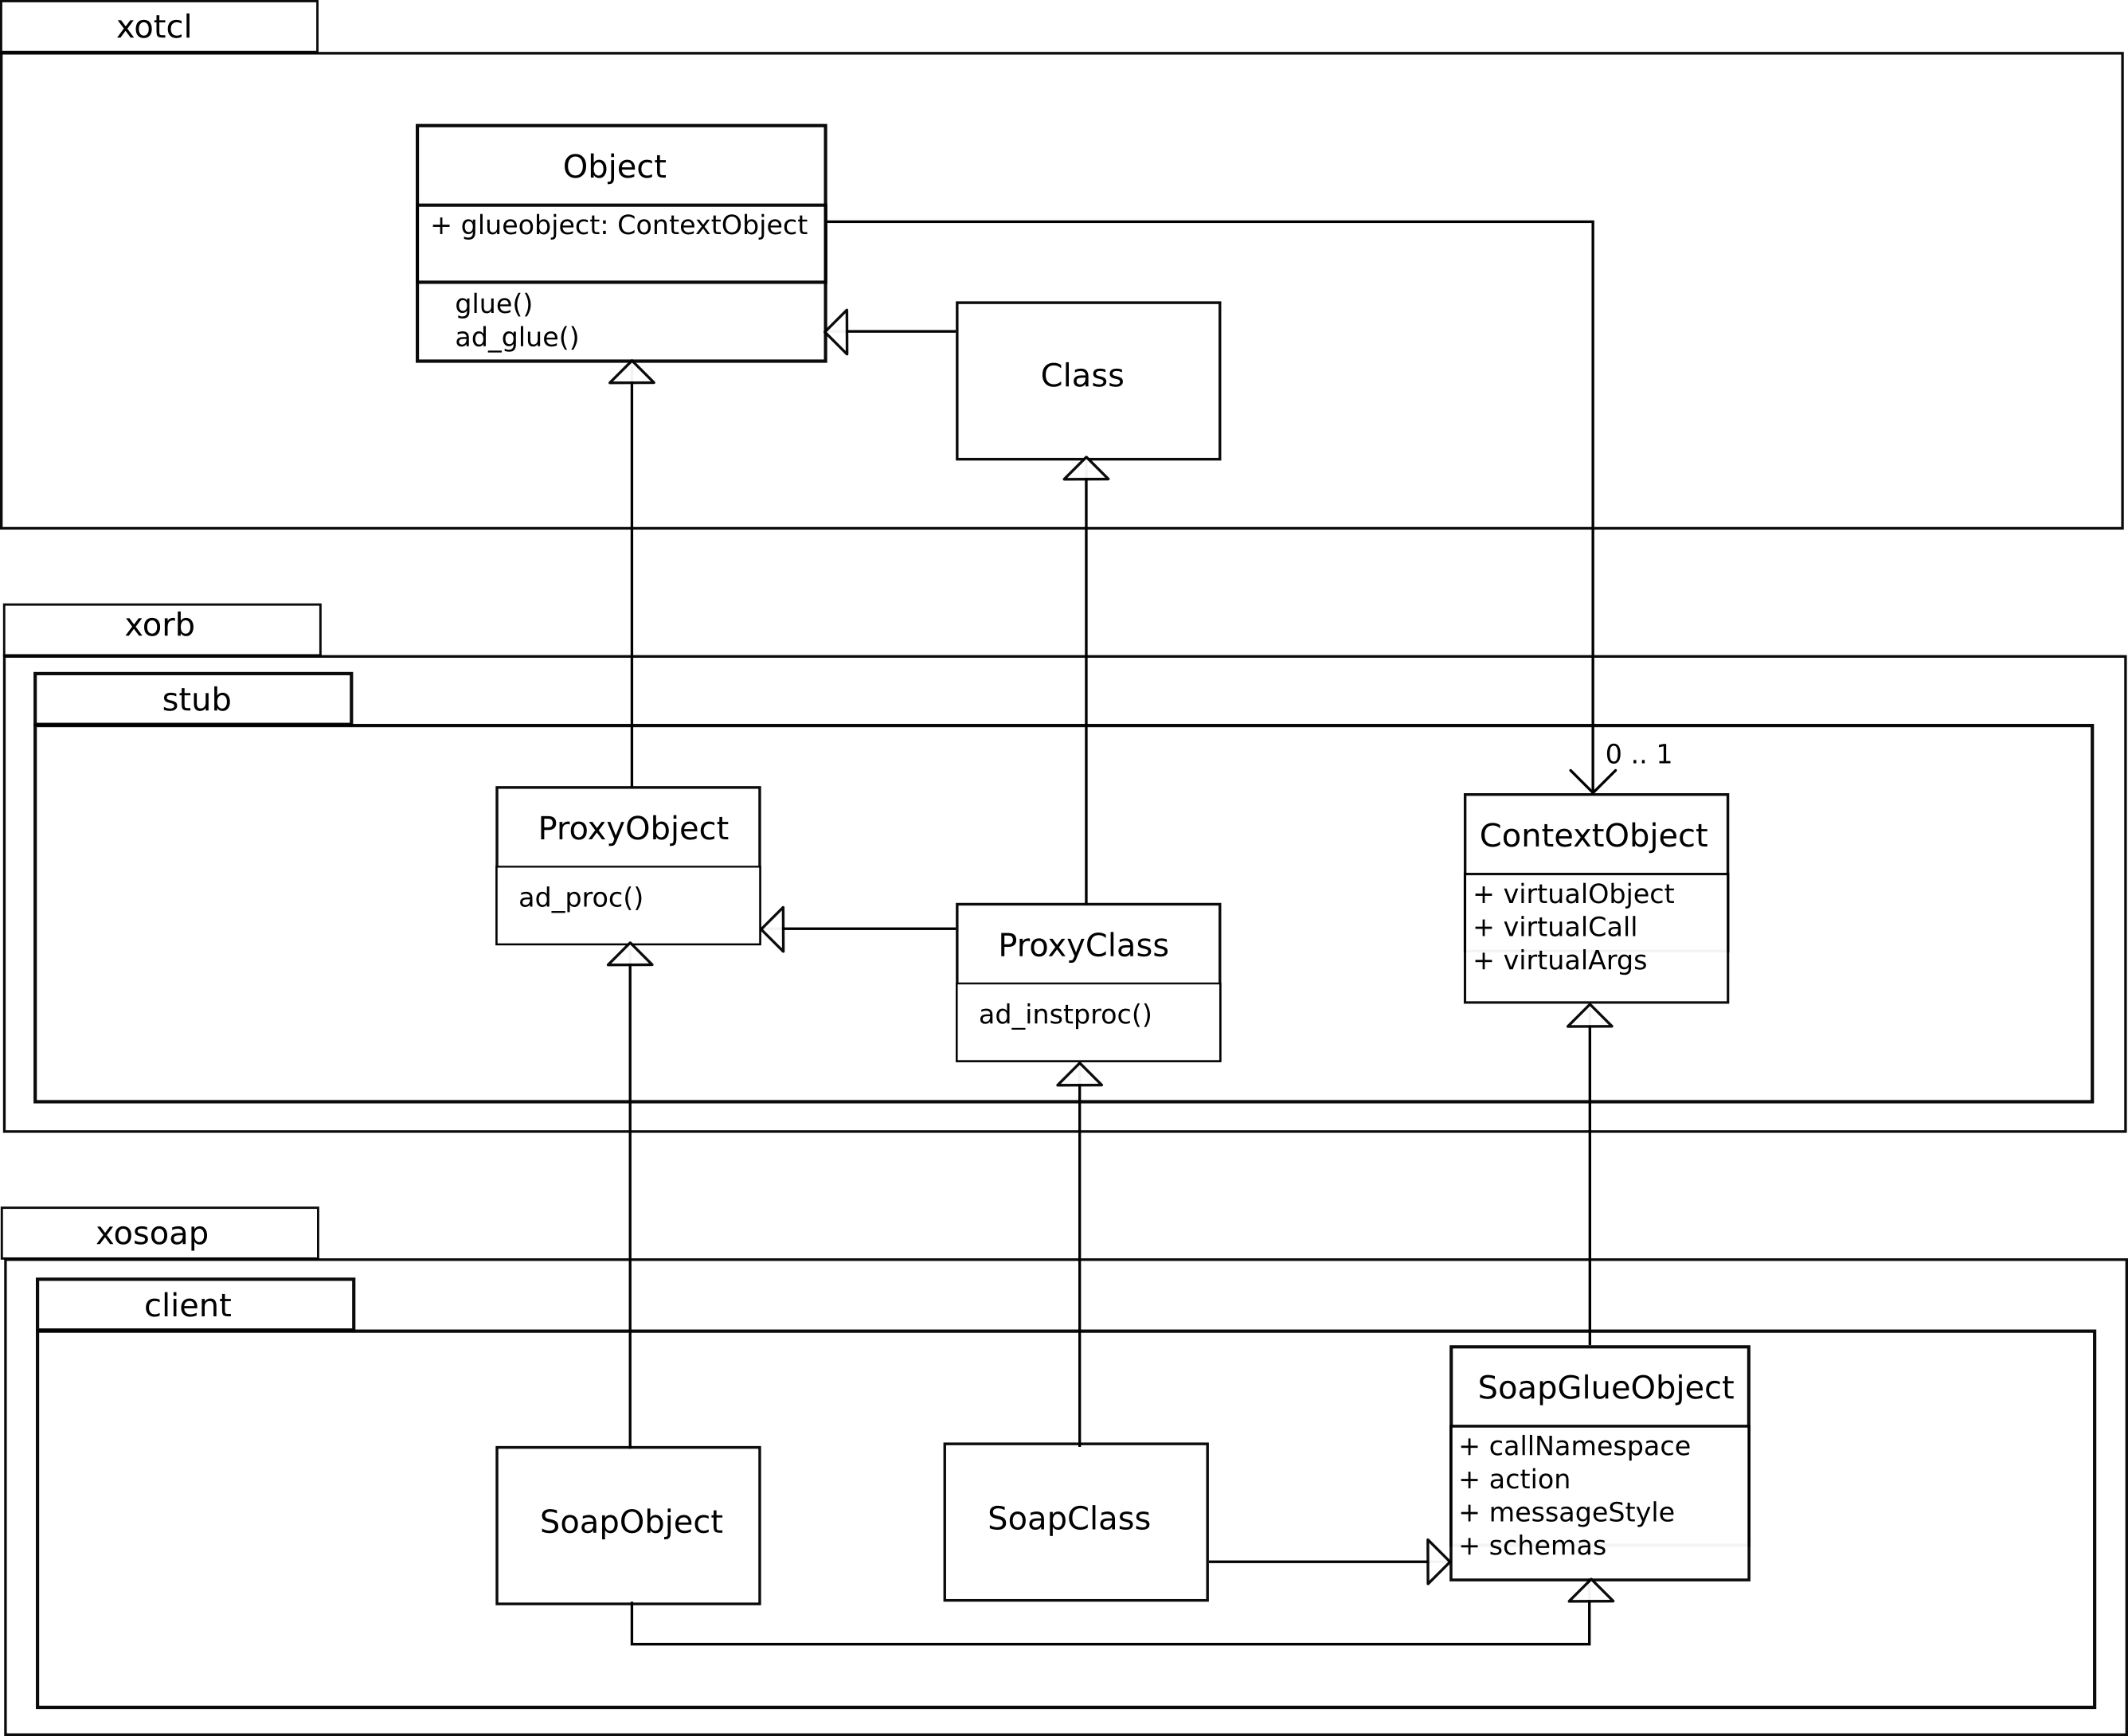
\includegraphics[width=0.75\textwidth]{img/xorb-xosoap-consumer-interface.png}
\caption{Class diagram of interface entities}
\label{fig:advanced:interface:1}
\end{center}
\end{figure}

The \emph{medium-level interface} is already familiar to the reader when reviewing the quick start 
section. It is provided by xorb and more or less introduces two xorb-specific idioms, 
i.e. ::xorb::stub::ProxyObject and ::xorb::stub::ProxyClass. While they inherit all capabilities of the low-
level interface, they provide additional facilities to create and use proxy objects. A glimpse at Figure \ref
{fig:advanced:interface:1} reveals that they overwrite the methods \emph{ad\_proc} provided 
by ::xotcl::Object and \emph{ad\_instproc} ::xotcl::Class. This already suggests that proxy interfaces can 
now be declared in a slightly different manner than by glue/ad\_glue. While you can still revert to the 
former, ad\_proc and ad\_instproc allow for interface descriptors with method bodies. When looking at 
Listing , you might notice that the argument containing the method body declarations is empty 
(corresponds to an empty Tcl string). For the sake of simplicity, we did not introduce a notable feature of 
the medium-level interface at that stage that we refer to as \emph{proxy templates}. For a primer on this 
concept and examples see Section \ref{sec:advanced:template}.

The \emph{high-level interface}, as can been seen from Figure \ref{fig:advanced:interface:1}, is a purely 
protocol plug-in-specific one. As for xosoap, we provide two intregating 
idioms: ::xosoap::client::SoapObject and ::xosoap::client::SoapClass inherit and expose and combine 
properties of glue objects and proxy clients in one. This allows for an abbreviated and compact writing of 
SOAP client code, with all facilities introduced by lower interface levels. For an introductory example see 
the quick start section on xosoap (see Section \ref{sec:quickstart:xosoap}) and, in particular, Listing \ref
{lst:quickstart:xosoap:3}.

 \subsection{Proxy templates}\label{sec:advanced:template}
Proxy templates or rather template methods on proxy objects follow an primary intention: Extending the 
use of pure interface descriptors to full-featured methods that allow to pack program logic along with a 
call abstraction in a single method body. Our intention can be best summarised when following the idea 
of the Template Method pattern as documented by \cite{gof:1994}. As the term template suggests, there 
might be scenarios that integrate call abstraction, or in our remoting scenario simply remote calls, in 
more complex (i.e. multi-step) behaviour. This is, certainly, also realisable with the lower-level interface. 
However, it would require another construct, either a proc, or a subclass etc., that combines the general 
behaviour and the invocation references to the abstracted calls. By means of proxy template methods as 
introduced by the medium-level interface you can know write template code and invocations of 
abstracted calls in the same method block, making encapsulation in this respect more seamless. A 
primary, and still easily graspable example are conditional invocations of abstracted calls. Let's take the 
following example of Listing \ref{lst:quickstart:xosoap:2} where we simply rewrite lines 16 -- 21. This 
yields the following (see Listing \ref{lst:quickstart:xosoap:5} for the complete example): 

\lstinputlisting[breaklines=true,numbers=left,frame=single,basicstyle=
\footnotesize,firstline=16,lastline=28]{../examples/xosoap/example-04-soap-consumer.tcl}

We draw your attention to the last argument of the ad\_proc call which perfectly resembles the 
declaration of a method body. The exemplary condition we introduce here is only to simplistic but 
delivers the message. You might have noticed that the floating point number used in the EchoClient/
EchoService example corresponds to the decimal representation of the golden ratio phi. We, now, in our 
proxy template method, introduce a constraint which limits the value space accepted to all decimals that 
round to the same integer as the most accurate decimal expansion of the golden ratio, given by the 
formula \begin{math} (1 + \sqrt{5}) / 2\end{math}. If, and only if this value validation is passed, we want 
the remote call to be invoked. At this point, you might have realised that the ::xotcl::next command is the 
forwarder to the actual proxy method. 

Now, once you got the main idea behind this example, take a closer look  at the declaration of 
arguments in line 17. You might notice that there is a slight but important modification of how the 
argument inputFloat is specified. In fact, we added an additional \emph{check option 'glue'} which is 
mandatory as soon as you provide a non-empty method body to either ad\_proc and ad\_instproc. There 
are two reasons for this requirement: First, regarding concepts and clarity for you as developer, you are 
now specifying two method records (i.e. set of arguments plus check options)  within one single step, on 
the one hand, the record for the decorating method (the proxy template method) called "echoFloat" and, 
on the other han, the actual stub method "echoFloat". We, therefore, distinguish between an inner and 
and outer record. Both records might be identical but not necessarily. Second, regarding internals, it is 
required to explicitly distinguish between elements of either record. Lets have a look at another variation 
of the previous example (see Listing \ref{lst:quickstart:xosoap:6}):

\lstinputlisting[breaklines=true,numbers=left,frame=single,basicstyle=
\footnotesize,firstline=16,lastline=34]{../examples/xosoap/example-05-soap-consumer.tcl}

Referring to lines 17-21, we extended the method's record by an additional non-positional argument and 
two positional ones. In fact, "annotating" a non-positional argument with 'glue' assigns it to be member in 
the proxy or stub record, while all the others, especially the other non-positional arguments, won't be 
interpreted as elements of the proxy interface. At the same time, you will be able to use equally named 
variables containing the arguments' values in the scope of the proxy template method. The final call to 
the proxy object by means of the template method might take the following form:

\lstinputlisting[breaklines=true,numbers=left,frame=single,basicstyle=
\footnotesize,firstline=37,lastline=41]{../examples/xosoap/example-05-soap-consumer.tcl}

Apart from the constraint scenario, template methods also proof useful when you (for whatever reason) 
want to deviate from the proxy interface (i.e. the inner record). This might true in the following cases:
\begin{itemize}
\item In case you need to mangle the argument values before being passed to the remote method, or
\item if you do not expose all arguments stipulated by the proxy interface (i.e. the inner record) in the 
outer record.
\end{itemize}

In the following variation of an initial listing (see Listing \ref{lst:quickstart:xosoap:5}), we give provide an 
example for the first case. Let' see:

\lstinputlisting[breaklines=true,numbers=left,frame=single,basicstyle=
\footnotesize,firstline=29,lastline=33]{../examples/xosoap/example-06-soap-consumer.tcl}

Here, we simply take the inbound value for inputFloat and increase it by 1. This updated value should 
then be passed to the remote method to be communicated to the remote point. Two important aspects 
should be retained from this snippet: First, if you do so, you have to explicitly append argument-value 
pairs to ::xotcl::next. Otherwise, ::xotcl::next, if called without any appended terms, passes on the last 
argument list on the call stack. Second, if you decide to do so, you have to provide all arguments 
to ::xotcl::next that are required by the method shadowed by ::xotcl::next. Required arguments are both 
non-positional arguments flagged 'glue' or 'required' and positional arguments with no default values in 
the record declaration.


\begin{hints}
\item We assume that your are familiar with the basic mechanism of inheritance XOTcl delivers to you. If 
you are new to XOTcl or its conceptual "sponsors" such as CLOS etc., you might want to consider 
studying the relevant sections.
\item You might want to give it a try. Just edit the last line of the example outlined above and change the 
value passed as "inputFloat" so that it once validates correctly and once fails.
\end{hints}

Using ::xotcl::next in this setting is both a slight redefinition of its semantics in view of XOTcl inheritance, 
and a pointer to the internal implementation of our proxy templates or proxy template methods: The 
declarative information passed to ad\_proc or ad\_instproc is used both (a) to specify a proxy method 
and register it with invocation infrastructure and (b) to create a decorator to the actual proxy object in 
terms of a XOTcl mixin class. This decorator hosts the method body as declared with ::xotcl::next 
resolving to the shadowed proxy method.

\begin{figure}[htbp]
\begin{center}
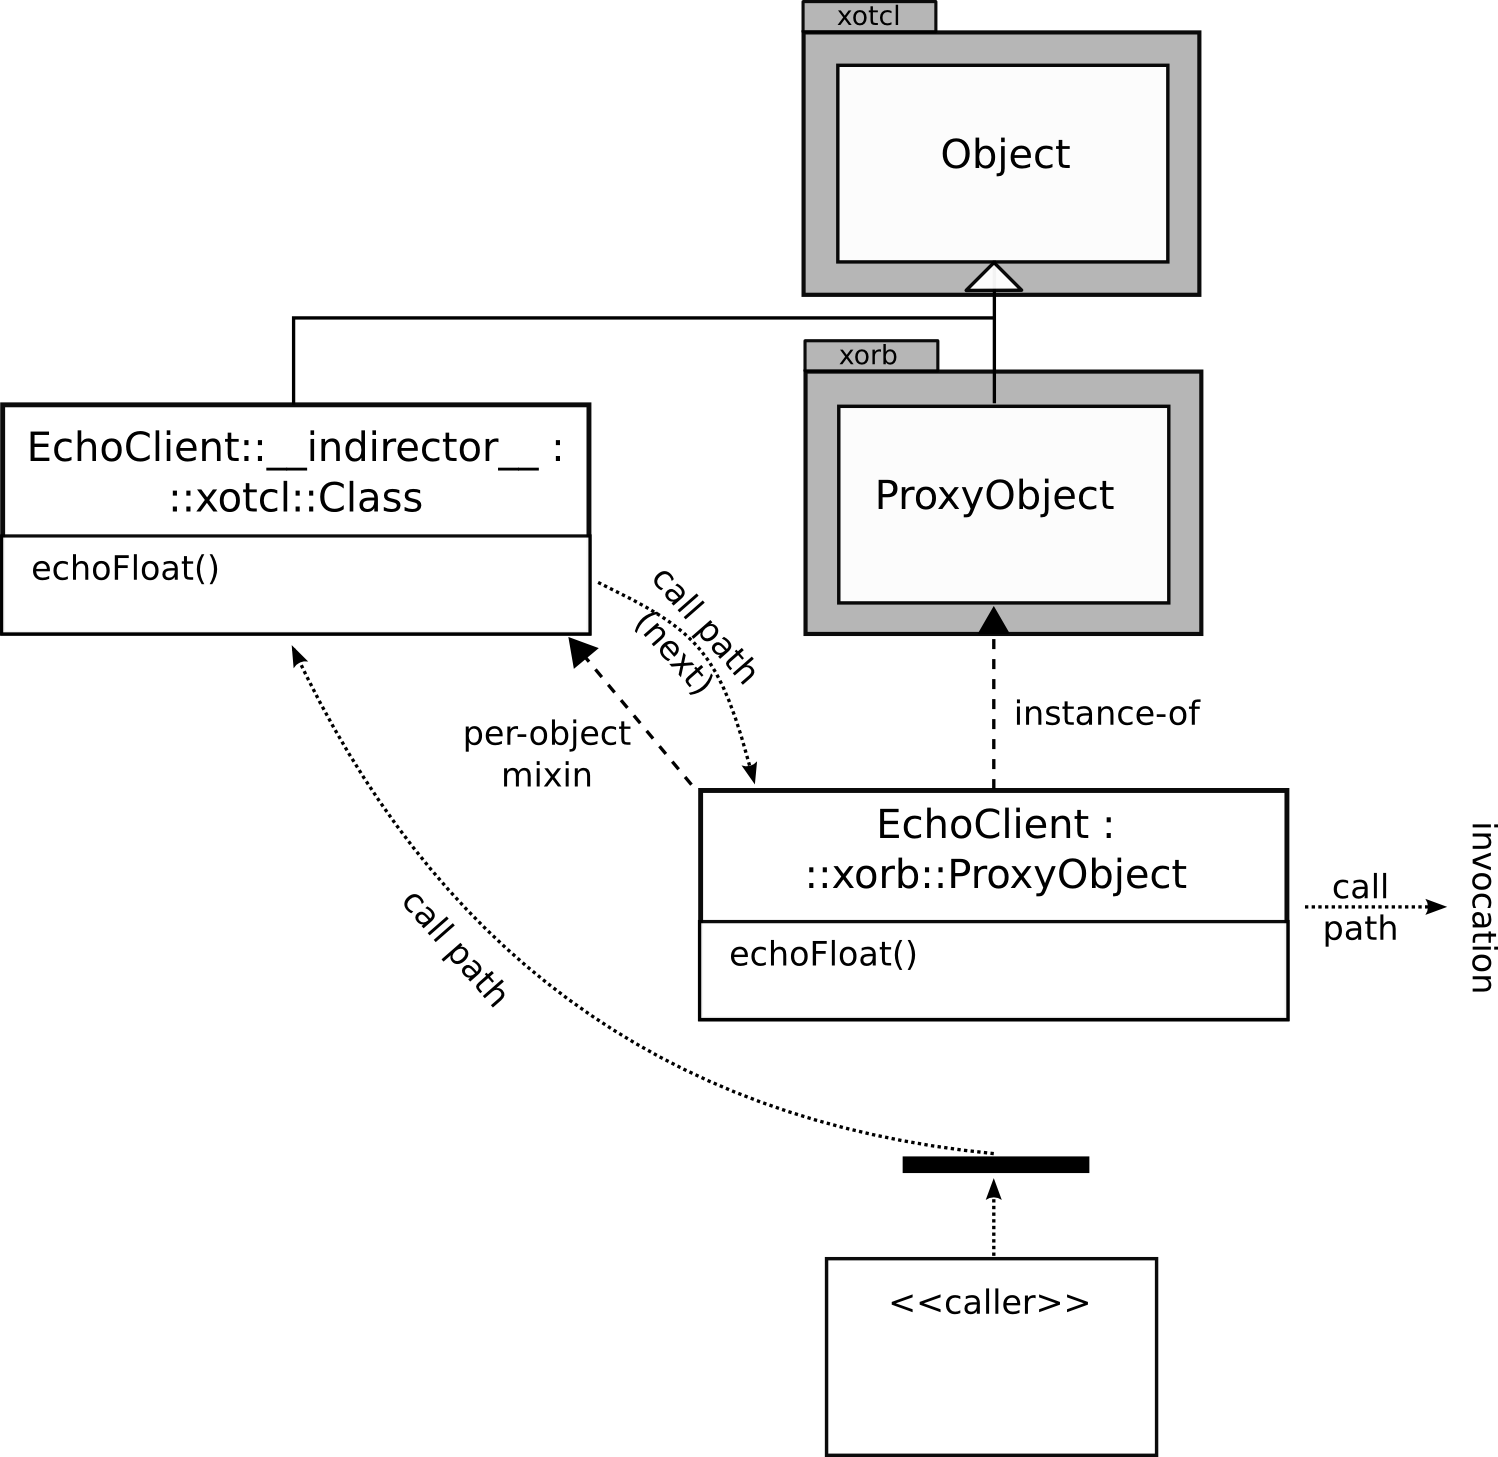
\includegraphics[width=0.5\textwidth]{img/proxy-template.png}
\caption{Call indirection as used for proxy templates}
\label{fig:advanced:templates:1}
\end{center}
\end{figure}

Figure \ref{fig:advanced:templates:1} aims at sketch the internals of proxy template methods and the 
behaviour shown above. Again, we assume some familiarity with XOTcl concepts, especially mixins as 
XOTcl's realisation of abstract subclasses. The main messages from Figure \ref{fig:advanced:templates:
1} are the following:
\begin{itemize}
\item Calls upon objects that mixin classes are registered with are indirected according to a certain order 
of precedence, visualised by the call path in Figure  \ref{fig:advanced:templates:1}.
\item What previously has been referred to as outer interface is the method record of echoFloat defined 
on the mixin class (i.e. \lstinline!::EchoClient::__indirector__!). The inner record refers to the record 
declaration of echoFloat of EchoClient.
\item The original or native call path in XOTcl would continue along the inheritance and realisation 
(instantiation) path, involving e.g. ProxyObject and Object in Figure  \ref{fig:advanced:templates:1}. 
However, in the context of proxy templates, the call as such leads to the actual invocation of the 
abstracted call.
\end{itemize}
  \subsection{Glue objects}\label{sec:advanced:xorb:gobjects}
  \subsubsection{What is the idea of glue objects?}\label{sec:advanced:xorb:gobjects:what}
  \subsubsection{Why do we use context objects in xorb and its plug-ins?}\label
{sec:advanced:xorb:gobjects:why}
  \section{Internals}\label{sec:internal}
  \subsection{What are "service contracts"?}\label{sec:internal:contracts}
  % call abstractions
  % interface descriptions
  \section{Feature sets}
  \subsection{xorb}
  \subsection{xosoap}
  \section{Roadmap}
   \subsection{xorb}	
  \subsection{xosoap}
  \section{Appendix} 
  \subsection{Examples - xosoap} 
 \lstinputlisting[breaklines=true,numbers=left,label=lst:quickstart:xosoap:2,frame=single,basicstyle=
\footnotesize,caption=A simple SOAP client]{../examples/xosoap/example-01-soap-consumer.tcl}
  \lstinputlisting[breaklines=true,numbers=left,label=lst:quickstart:xosoap:3,frame=single,basicstyle=
\footnotesize,caption=An even simpler SOAP client]{../examples/xosoap/example-02-soap-consumer.tcl}
    \lstinputlisting[breaklines=true,numbers=left,label=lst:quickstart:xosoap:4,frame=single,basicstyle=\footnotesize,caption=An XOTcl Object as SOAP client]{../examples/xosoap/example-03-soap-consumer.tcl}
        \lstinputlisting[breaklines=true,numbers=left,label=lst:quickstart:xosoap:5,frame=single,basicstyle=\footnotesize,caption=Using proxy templates/ template methods (I)]{../examples/xosoap/example-04-soap-consumer.tcl}
     \lstinputlisting[breaklines=true,numbers=left,label=lst:quickstart:xosoap:6,frame=single,basicstyle=\footnotesize,caption=Using proxy templates/ template methods (II)]{../examples/xosoap/example-05-soap-consumer.tcl}
     \lstinputlisting[breaklines=true,numbers=left,frame=single,basicstyle=
\footnotesize]{../examples/xosoap/example-07-soap-provider-init.tcl}
 \newpage
 \bibliography{/Users/ssoberni/Documents/doc/diss/thesis}
 \newpage
\printindex
    \end{document}
    
    %        In the following section, I assume that you have OpenACS 5.1+ or DotLRN 
%        2.1.3+ up and running on your localhost at the default port 
%        80.\footnote{The version requirements result from the actual 
%        requirements for the underlying \href{http://www.xotcl.org}{XOTcl} 
%        extensions to OpenACS, see e.g. 
%        \href{http://media.wu-wien.ac.at/download/README-xotcl-core}{XOTcl 
%        installation readme for OpenACS}.} When referring to code artefacts, I
%        will skip namespaces used (e.g. xosoap::*) for the sake of readability.
%        As xoSoap aims at providing remoting 
%        for \href{http://www.xotcl.org}{XOTcl} objects deployed within the 
%        OpenACS/ DotLRN framework, in a first step, you have to make sure that 
%        XOTcl extensions to OpenACS are properly installed for your OpenACS/ 
%        DotLRN instance: \subsubsection{Introducing OO to OACS} Upgrading your 
%        OACS instance to the powerful OO features of 
%        \href{http://www.xotcl.org}{XOTcl} is fairly straight forward and 
%        involves three steps: First, you have to add the 
%        \href{http://www.xotcl.org}{XOTcl} Tcl-extension library as module to 
%        your AOLServer installation. Then, you are required to patch your 
%        OpenACS core, mainly to allow XOTcl's auxiliary facilities to be loaded 
%        at the very beginning of the bootstrap loading process (see 
%        \href{http://openacs.org/forums/message-view?message_id=313344}{TIP 
%        #87} for details on merging XOTcl extensions with the OACS core). 
%        Complete and thorough upgrading instruction come with the XOTcl 
%        extension distribution, you find them at 
%        \href{http://media.wu-wien.ac.at/download/README-xotcl-core}{http://media.wu-wien.ac.at/
download/README-xotcl-core}. 
%        Note: These instructions do not only cover the set up process for XOTcl 
%        fundamentals but also for some jelly beans, e.g. a threaded profiling 
%        environment etc.\footnote{The family of XOTcl-based OACS extensions 
%        grows rapidly: Included in the XOTcl distribution, there is an advanced 
%        repository management component (XOTcl-Note), Gustaf Neumann recently 
%        came up with a Wiki extension for OACS called
% 	        \href{http://openacs.org/forums/message-view?message_id=334982}{xoWiki}.} 
%        xoSoap only requires the basic bundle of XOTcl artefacts, i.e. the 
%        AOLServer module, the auxiliary XOTcl core package and the two patches 
%        to the OACS core. All of these can be retrieved directly from 
%        \href{http://media.wu-wien.ac.at/download/}{http://media.wu-wien.ac.at/download/}. 
%        At the time of writing this document, these were the following files or 
%        files' versions:
%          \begin{itemize}
%            \item
%            \href{http://media.wu-wien.ac.at/download/xotcl-1.3.8.tar.gz}{xotcl-1.3.8.tar.gz}
%            \item
%            \href{http://media.wu-wien.ac.at/download/xotcl-core-0.19.apm}{xotcl-core-0.19.apm}
%            \item
%            \href{http://media.wu-wien.ac.at/download/acs-api-documentation-procs.patch}{acs-api-
documentation-procs.patch}
%            \item
%            \href{http://media.wu-wien.ac.at/download/acs-bootstrap-installer.patch}{acs-bootstrap-
installer.patch}
%          \end{itemize}
%            Get these and follow the relevant instruction in 
%            \href{http://media.wu-wien.ac.at/download/README-xotcl-core}{README-xotcl-core}.
% 	      \subsubsection{Setting up xoSoap}
%            xoSoap comes in an APM flavour and can therefore be easily 
%            incorporated into your OpenACS installation:
%       \begin{enumerate}
%         \item Grab the current xoSoap distribution package from
%         \href{http://stefan.thinkersfoot.net}{http://stefan.thinkersfoot.net}
%         and load the xoSoap package (either assisted by APM package manager or 
%         manually) e.g.:
%        \lstset{basicstyle=\small}
% 		\begin{lstlisting}[language=bash,breaklines=true,label=lst:loadpkg]         
%         cd <path-to-your-oacs-instance>/packages 
%         # (e.g. /var/lib/aolserver/<instance/packages) 
%         wget http://stefan.thinkersfoot.net/file_download/4          
%         \end{lstlisting} 
%         Alternatively, you can directly "load" the package by using the APM 
%         package manager that allows for retrieving a package from your local 
%         filesystem or a remote web repository. To do so, go to 
%         /acs-admin/apm/package-load and follow the instructions.
%         \item Install xoSoap: Depending on whether you use or stick with the 
%         APM package manger, either go to /acs-admin/apm/packages-install or 
%         simply /acs-admin/install. xoSoap will then be mounted under /xosoap.
%         \begin{enumerate}
%           \item In the former case, select the check box representing the 
%           loaded xoSoap package and continue with "Next". Installation should 
%           be completed right away as there is no database / data model 
%           modification/ extension necessary.
%           \item In the latter case, select "Install from local" and then the 
%           "Service" branch of locally loaded packages available for 
%           installation. xoSoap should then be properly listed.
%         \end{enumerate}
%           \item Restart the AOLServer.
%           \item Verify that xoSoap is correctly initialised.
%	         \begin{enumerate}
%                   \item First, check /logs/error.log for some basic 
%                   notifications issued by xoSoap upon initialization: xoSoap 
%                   informs you about hooking itself into the request processor 
%                   chain, therefore look for a notification that says "[xoSoap] 
%                   preauth filter set for post requests debarking at /xosoap*."
%                   Besides, make sure that all library files (*-procs.tcl) were
%                   loaded appropriately by taking a sample of messages posted by the
%                   bootstrap loader. Watch out for notifications saying
%                   "Loading" or "Loaded packages/xosoap/<procs-file>" and possible
%                   sourcing errors.
%                   \item Go to /xosoap. There, you are supposed to find some 
%                   basic information about services (XOTcl objects) hosted and 
%                   registered for remoting (see Figure \ref{fig:hideout}). 
%                   Note: You will find information about a sample service that 
%                   comes with the xoSoap distribution named SqiTarget. Please, 
%                   refer to Section \ref{sec:publish} for more details.
%	         \end{enumerate}
%       \end{enumerate}
%                   \begin{figure}[htb] \centering
%\includegraphics{img/hideout}
%\caption{xoSoap's hideout}
%\label{fig:hideout}
%\end{figure}
    
%So far you have got xoSoap up and running. At this point you will be briefed on
%how to create and publish your own web service. Some basics:
%\begin{itemize}
%\item Usually SOAP frameworks distinguish between creating or declaring a
%service and deploying it. Under its roof, xoSoap does the very same. However, the 
%deployment step does not require any efforts by you, in fact, it is not even 
%visible at first sight. This is due to the fact that the deployment logic
%is encapsulated by the actual service syntax that you have to deal with
%(see Section \ref{sec:design}).
%\item Currently, the service declaring code is supposed to be placed into
%*-init.tcl files in your package. As xoSoap is loaded in the first bootstrap run
%that sources all *-procs.tcl files, it is not guaranteed that you can make use
%of xoSoap facilities in your procs-files. However, you are not limited to store
%your services in the native xoSoap package /tcl directory. Feel free to extend
%your (existing) packages by xoSoap services.
%\item Take a closer look at your xoSoap's library directory (i.e.
%<...>/packages/xosoap/tcl): There, you will find an examples-init.tcl
%file that comes with a small sample service, called Poem. I will closely follow
%this service example when outlining the process of service creation below.
%\end{itemize}
%Let's break it down into smaller bits and pieces:
%\begin{enumerate}
%  \item Create a custom namespace hosting your service declarations (Note:
%  xoSoap does not impose any restrictions on the usage of namespaces):
%    \lstset{basicstyle=\small}
% 		\begin{lstlisting}[language=tcl,breaklines=true,label=lst:declarens]         
%         namespace eval services {
%         # service declaration
%         }         
%         \end{lstlisting}   
%\item Then, you have to create the actual service from the Service 
%meta-class. Note that creating a xoSoap service does not differ from writing 
%XOTcl code as such. So if you are familiar with basic concepts of XOTcl 
%(meta-classes, object properties / parameters etc.) skip the next few steps. 
%Defining a service is done by declaring a XOTcl class. The service skeleton, a 
%XOTcl meta-class, provides for (1) the registration of the service with the 
%Invoker in several steps, (2) the definition of a lifecycle model for your 
%service (i.e. either static / persistent or per-request) and (3) the enclosure 
%or "hoarding" of service methods. The following line creates a new service
%called "Poem": 
%\lstset{basicstyle=\small}
% 		\begin{lstlisting}[language=tcl,breaklines=true,label=lst:declarservice]         
%         ::xosoap::Service Poem     
%         \end{lstlisting}   
%\item For the moment, the Poem service is completely disrobed, it does not come
%with any service-specific method defined upon it. Therefore, the service does
%not expose any functionality to the outer space. By adding any number of methods
%or instprocs to the newly created class, you can provide for these. The
%following lines attach functionality to the class' instances, the actual service
%objects. In the Poem example included in the distribution (see
%examples-init.tcl) the method actual implements a simple echo service, i.e. it
%returns a steadily growing vers. In other words, the object accumulates
%statements collected from the requesting clients ("statement" argument) and
%returns the current state to the request-issueing clients.
%\lstset{basicstyle=\small}
% 		\begin{lstlisting}[language=tcl,breaklines=true,label=lst:declarservice]         
%         Poem instproc getPoem {statement} {         
%         	# method's body         
%         }   
%         \end{lstlisting}  
%\item The two line blocks above give you a rudimentary but fully functioning
%service that can be called from a remote or local SOAP client. However, there
%are many refinements to consider:
%\begin{itemize}
%  \item Lifecycling: This refers to the design decision on the time-to-live for
%  service objects. Are they supposed to be creately only once, upon AOLServer /
%  OACS intialisation, stay alive and are reused for handling requests by several
%  requestors, or do you want each request / connection thread to be served by a
%  new or rejuvenated object. Both styles, referred to as "static instance" and
%  "per-request instance", allow for realising different application scenarios
%  (see Section \ref{sec:design} for a more thorough discussion). xoSoap leaves
%  the decision to you, by setting the optional lifecycle parameter of 
%  ::xosoao::Service either to 0 (per-request flavour; default) or 1 (static
%  instance). The Poem service declaration above gives you
%  short-living\footnote{Note: "Short living" is not the correct wording as it
%  turns
%  out to be relative to the time frame it takes for a servant object to process
%  an invocation task. In fact, "short-living servants" should be rephrased
%  "lemming servants" as their meeting-the-end is imposed forcefully.} service
%  objects (also referred to as servants), the following modification stretches
%  its time-to-live. If not the clear for the moment, testing will the Poem echo
%  service will give you illumination (see \ref{}): 
%  \lstset{basicstyle=\small}
% 		\begin{lstlisting}[language=tcl,breaklines=true,label=lst:declarservice1]         
%         ::xosoap::Service Poem -lifecycle 1  
%         \end{lstlisting}     
%\item Activation: Activation per se does not only refer to initialising an
%servant's inner state in a pre-defined manner, but might involve various tasks.
%At this point we stick with its limited scope, i.e. initialisation of an
%object's state. By defining a custom constructor method (the \textit{init}
%instproc), you can controll the (1) initial creation process upon the first
%request and (2) --- in case of per-request instances --- their regeneration:
%\lstset{basicstyle=\small}
% 		\begin{lstlisting}[language=tcl,breaklines=true,label=lst:declarinit]         
%    Poem instproc init {} {	
%		my set result "Rose"	
%}
%         \end{lstlisting} 
%The block above creates a constructor that is called at the time of a
%servant's creation (instantiation of the service class) and sets the initial
%vers of the poem to be constructed. Statements by the requesting clients will
%then be appended to this initial state.
%\item Hoarding: By default, any method you define on the service class will be
%exposed for remote invocation. In order to give you more control about the dis-
%or, actually, the enclosure of functionality exposed, Service
%meta-class provides you with the parameter "hoard". By passing a list of method
%names to this parameter you can define an interface "ad negativum" and prevent
%methods, such as the constructor, to be invokable remotely. So after this
%refinement we end up with the following service class declaration:
%\lstset{basicstyle=\small}
% 		\begin{lstlisting}[language=tcl,breaklines=true,label=lst:declarservice2]         
%    ::xosoap::Service Poem -hoard [list init] -lifecycle 1
%         \end{lstlisting} 
%\end{itemize}
%\item Save your coding artefact and restart the AOLServer.
%\item Testing: xoSoap was developed with and tested against two SOAP frameworks
%that can be used with (XO)Tcl: \href{http://tclsoap.sourceforge.net/}{tclsoap}
%(version 1.6.7) and \href{http://www.cs.fsu.edu/~engelen/soap.html}{gSoap}, a
%SOAP suite for C/C++ that can easily be extended by Tcl bindings. For the
%moment, I provide a few-liner sample tclsoap consumer in this distribution and for
%the included Poem echo service (see <...>/xosoap/tcl/doc/poem.tcl). I therefore
%assume that you know how to set up tclsoap properly:
%\lstset{basicstyle=\small}
% 		\begin{lstlisting}[language=tcl,breaklines=true,label=lst:declarservice2]         
%package req SOAP

%SOAP::create getPoem \
%        -uri "urn:xmethods-getPoem" \
%        -proxy "http://localhost/xosoap/services/SqiTarget" \
%        -params { "statement" "string"}

%puts [getPoem "is a rose"]

%         \end{lstlisting} 
%\item Enjoy watching the creation of the widely known part of Gertrude Stein's
%Sacred Emily poem written in 1912.
%  \end{enumerate}
%  \subsection{Mangling messages using Interceptors}\label{sec:usinginterceptors}
%Now you can easily deploy your own web services or recast existing OpenACS 
%functionality written in XOTcl in a service-style manner. xoSoap gives you the
%opportunity to extend its functionality according to your needs, i.e. the
%invocation procedure, by means of invocation interceptors, also known as
%"handlers" in other web service frameworks. Although this feature is still
%maturing, you can plugin in basic logging, monitoring, debugging or
%security-relevant features (authentication) by writting your own interceptors.
%For the moment, xoSoap
%distinguishes between interceptors that listen at the request flow (incoming
%messages, RequestInterceptors) and those listening at the response flow
%(outgoing messages, ResponseInterceptors):
%  \section{xoSoap sandboxes}
%  \subsection{Implementing the Simple Query Interface (SQI)}
%  \section{Dissecting xoSoap}
%  \subsection{Design overview}\label{sec:design}
%  \subsection{Little design gems}
%  \subsubsection{Intercepting message flows}
%  In Section \ref{sec:usinginterceptors} I introduced to you the usage of
%  interceptors / handlers to listen at the flows of request and response in
%  order to plug-in additional pre- and post-invocation functionality. The
%  following section wants to give some insights on the actual design of
%  interception in xoSoap. While reading, you might refer to the code
%  documentation as well, providing more details on each of the code artefacts
%  involved in the realisation of interception. The top-level concept is the
%  interception \textit{scope}, i.e. the scope for application of an interceptor
%  with respect to threads. Certain scenarios (e.g. caching) require
%  state-preserving interception while others can equally be realized at the
%  level of each connection (thread). Therefore, xoSoap currently comes with two
%  interception scopes, a connection scope and an invoker scope. This is
%  realised by attaching a chain of interceptors to core objects in either
%  thread sphere (see Figure \ref{fig:icpt-design}). Interceptor {chains} make
%  use of one of XOTcls interception techniques, mixins, i.e. per-object mixins to
%  more precise.\footnote{Please refer to the mixin-section of the \href{http://media.wu-wien.ac.at/doc/
tutorial.html#mixins}{XOTcl
%  manual} for more details in per-object and per-class mixins.} The XOTcl class
%  InterceptorChain serves as superclass of both the MessageHandler and the
%  Invoker class. Upon instantiation of MessageHandler (in the main / blueprint
%  and therefore each connection thread) or Invoker (in the invoker thread), the
%  constructor of InvocationChain is called and nests two \textit{flow} objects,
%  Request- and ResponseFlow, into the two objects just created. As XOTcl
%  mixins allow for propagation of specific method calls\footnote{This happens
%  by extending and therefore along the so called \textit{next}-path, see
%  \href{http://media.wu-wien.ac.at/doc/tutorial.html#mixins}{XOTcl
%  manual}.}, calls upon the handleRequest / handleResponse methods provided by
%  both MessageHandler and Invoker are redirected, first to the shadowed methods
%  of InvocationChain, i.e. their common superclass. 
%  
%   \begin{figure}[htb] \centering
%\includegraphics{img/interceptor-design}
%\caption{Intercepting architecture -- Scopes, Chain, Flows, Bouncers}
%\label{fig:icpt-design}
%\end{figure}
%  
%  The latter then administers the call to the respective nested
%  flow objects that actually have mixed-in the inceptor mixin classes (the
%  registration procedure is outlined later in this section). This redirection
%  along a method chaining (\textit{next}-) path is at the core of
%  interception as realised in xoSoap. Intercepting requests and responses might
%  come in two flavours, either intercepting-forwarding or
%  intercepting-bouncing. The latter is required by default in order to return
%  the result of a chain of interceptors, i.e. the mangled request / response,
%  back to the intially calling object / method, i.e. MessageHandler or Invoker.
%  Therefore interceptors can be written as flow \textit{bouncers}, they may
%  break a chain of interceptors by returning the status quo to the caller (see
%  Section \ref{sec:usinginterceptors}. xoSoap comes with two built-in flow
%  bouncers that are responsible for delimiter the list of mixins attached to a
%  flow object. In other words, they are in charge of closing request and
%  response flows and bounce the mangled request / response back to the calling
%  object (look for FlowBouncerForMessageChain and
%  FlowBouncerForInvokerChain in the source documentation). However,
%  this final bouncing involves different operations in either scope:
%  FlowBouncerForMessageChain (connection scope) forwards the request to
%  the invoker thread while FlowBouncerForInvokerChain initiates the
%  actual invocation procedure (see Figure \ref{fig:icpt-design}).
%  
%  \paragraph{Precedence order of interceptors}
%  In which precise order are interceptors enforced, i.e. can they intercept
%  requests / responses and mangle them? From your perspective as coder
%  of concrete interceptors it follows the principle of
%  "first-come-first-serve". To put it differently, what is declared first is
%  registered earlier in the respective chain and called first. Focusing xoSoap
%  internals, the precedence order derives from the order of the mixin list,
%  i.e. the list of mixin classes registered with a specific object. This list
%  of mixins can be altered in terms of a simple Tcl list\footnote{Refer to the
%  \href{http://media.wu-wien.ac.at/doc/tutorial.html#updateinterceptors}{XOTcl
%  manual}.} Each interceptor customly defined is simply appended to this list,
%  the two built-in bouncing interceptors, however, are made sticky at the very
%  end of the mixin list in order to make sure that chain does not become broken
%  at the very, very end. Custom bouncers are subject to the same precedence
%  strategy. Precedence is materialised by the underlying registration procedure.
%  
%  \paragraph{Registration procedure for interceptors} 
%  
%  The class InvocationChain includes a method register that handles the
%  hooking-in of newly declared interceptors, i.e. mixin classes. Registration
%  is realised in several steps, distributed among three artefacts:
%  \begin{enumerate}
%        \item The meta-class Interceptor provides for the selection of
%        the targeted scope in which the new interceptor is to be placed. The
%        constructor of Interceptor first collects the value of the
%        \textit{-scope} parameter (0 by default) and applies a switch: In case
%        of 0, the interceptor is passed to the addInterceptor method exposed by
%        the concrete object derived from MessageHandler. The object
%        inherits the registration method (addInterceptor) from
%        InvocationChain. In case of 1, i.e. the invoker thread is
%        targeted and the interceptor will apply to all incoming requests and
%        responses, the switch expression enforces a delayed registration.
%        Postponing the registration to the end of the intialization process is
%        necessary due to the current design of OACS's init process\footnote{See
%        \href{http://openacs.org/forums/message-view?message_id=324185}{OACS
%        forum} for a detailled discussion.}. This is achieved by queueing the
%        actual registration call on Invoker's addInterceptor method
%        with \lstinline[[language=tcl]!ad_after_server_initialization!.
%        \item The actual registration is performed by addInterceptor method
%        hosted by InterceptorChain. It is in charge of two tasks: (1)
%        As interceptors might either listen at the flow of requests or responses
%        or both, the have to be mixed-in accordingly, i.e. appended to the list
%        of mixin classes of either RequestFlow or ResponseFlow. Interceptors are
%        required to derive from either of the following or both "abstract"
%        superclasses: RequestInterceptor or / and
%        ResponseInterceptor. These prescribe the implementation of two
%        abstract methods, handleRequest or handleResponse. Upon registration,
%        addInterceptor performs a type check and registers each
%        Interceptor according to its superclass relationsships. (2)
%        Each flow has to be terminated by a flow bouncer. After successfully
%        registering a new Interceptor, addInterceptor provides for
%        re-appending of the built-in bouncer and re-initiating the mixin list. 
%      \end{enumerate}
%      
%       \begin{figure}[htb] \centering
%\includegraphics{img/interceptor-design-register}
%\caption{Intercepting architecture -- Registration & Precedence}
%\label{fig:icpt-design-register}
%\end{figure}
%  	 
%  \section{Benchmarking / Profiling}
%  \section{Known Issues}
%  \section{To-dos} 
